\documentclass[sigconf,review]{acmart}
\usepackage{booktabs}


\settopmatter{printacmref=false}
\setcopyright{none}
\acmConference[AgenticDev 2026]{International Workshop on Agentic AI for Next-Generation Software Development}{October 12, 2026}{Munich, Germany}
\acmISBN{}
\acmDOI{}

\newcommand{\ctx}{\texttt{context.md}}
\newcommand{\artifact}{\url{https://github.com/kerbelp/context-md}}

\authorsaddresses{}
\begin{document}

\title{The Repository Context Layer: A Git-Native Architecture for AI Coding Agents}

\author{Pavel Kerbel}
\authornote{Corresponding author. All authors are affiliated with Metatron Research (\url{https://getmetatron.com}); ORCIDs identify each author.}
\orcid{0009-0004-4679-1036}
\email{pavel@getmetatron.com}
\affiliation{\institution{Metatron Research}\country{}}
\author{Milana Kerbel}
\orcid{0009-0004-7893-9824}
\email{milana@getmetatron.com}
\affiliation{\institution{Metatron Research}\country{}}
\author{Vitali Abramov}
\orcid{0009-0007-0814-3822}
\email{vitali@getmetatron.com}
\affiliation{\institution{Metatron Research}\country{}}
\author{Liat Abramov}
\orcid{0009-0006-1601-146X}
\email{liat@getmetatron.com}
\affiliation{\institution{Metatron Research}\country{}}

\begin{abstract}
AI coding agents repeatedly rediscover project constraints, because repositories version code but not operating knowledge: the decisions taken, the alternatives rejected, the constraints found during execution. We introduce the \emph{Repository Context Layer} (RCL): the repository carries its own agent-facing context---versioned with the code, deterministically discoverable, consulted by contract, and writable by agents only under human review---in a minimal default format, \ctx{}. We evaluate the pattern in a pre-registered experiment on SWE-bench Verified. A frontier agent running the consult--execute--learn--promote lifecycle resolves held-out tasks sharing a constraint 14.6 percentage points more often (72.9\% vs.\ 58.3\%, paired $p=0.041$) while spending 32\% fewer tokens per resolved task. The benefit for a small local model depends on the context's author: frontier-written context improves its localization by 26 points ($p<0.0001$); its own lessons help not at all. Repository context should become a versioned software artifact, alongside code, tests, and documentation.
\end{abstract}

\begin{CCSXML}
<ccs2012>
<concept><concept_id>10011007.10011074</concept_id><concept_desc>Software and its engineering~Software creation and management</concept_desc><concept_significance>500</concept_significance></concept>
<concept><concept_id>10010147.10010178</concept_id><concept_desc>Computing methodologies~Artificial intelligence</concept_desc><concept_significance>300</concept_significance></concept>
</ccs2012>
\end{CCSXML}
\ccsdesc[500]{Software and its engineering~Software creation and management}
\ccsdesc[300]{Computing methodologies~Artificial intelligence}
\keywords{repository context layer, agentic software development, context.md, architecture decision records, agent memory, human-in-the-loop review}

\maketitle

\section{Introduction}
Coding agents crossed a practical threshold in 2024--2026: given a task, a modern agent can plan, edit, run tests, and iterate over hours with little supervision. What has not kept pace is the substrate those agents work on. A repository exposes its code, but not the reasoning that produced the code. The result is a familiar failure mode: an agent that writes competent code while re-proposing the library the team removed, violating an unwritten layering rule, or re-discovering, at some cost, a constraint a previous session had already found.

A concrete case: an agent reaches for an ORM to simplify a query, unaware the team removed ORMs months earlier because query opacity had broken an offline repair path. The decision lives in commit history and human memory---nowhere the agent consults. It writes reasonable code that a reviewer must catch, or that ships and regresses a constraint the project had already settled.

Practitioners mitigate this with a patchwork of mechanisms. Instruction files such as \texttt{CLAUDE.md}, \texttt{AGENTS.md}, and \texttt{.cursorrules} inject standing guidance into the prompt. IDE-level memories persist preferences per tool and per machine. Retrieval-augmented generation (RAG)~\cite{lewis2020rag} recalls similar text from an external index. Protocols such as MCP~\cite{mcp2024} standardize how agents reach external stores. Each helps; none yields a durable, reviewable, project-owned operating context that improves as work happens. Section~\ref{sec:background} examines why.

This paper formalizes an alternative that requires no new infrastructure: the repository carries its own operating context, versioned by Git, gated by code review, and updated as a routine part of every change. We call the pattern the \emph{Repository Context Layer} (RCL). A companion manifesto~\cite{manifesto} argues for the abstraction; this paper specifies and evaluates it. The contributions are:
\begin{enumerate}
\item a definition of the Repository Context Layer and its required properties (Section~\ref{sec:rcl});
\item a lifecycle with explicit branch, merge, and rollback semantics inherited from Git (Section~\ref{sec:lifecycle});
\item a deterministic context discovery specification and a minimal file format, \ctx{} (Sections~\ref{sec:discovery}--\ref{sec:format});
\item a design analysis of the contested choices: file granularity, append-only semantics, merge conflicts, hierarchy, and agent write authority, including the associated threat model (Section~\ref{sec:design});
\item a pre-registered evaluation on SWE-bench Verified showing the lifecycle improves a frontier agent's resolve rate and token efficiency on held-out constraint-sharing tasks, and that context-layer benefit requires an author more capable than the executor (Section~\ref{sec:eval}).
\end{enumerate}
Three findings preview the evaluation. First, the lifecycle works where it matters most: a frontier agent that recycles its own failure experience through a reviewed context file fixes a quarter more held-out bugs at a third less token cost per fix---for a strong model, the layer is self-financing. Second, whose knowledge it is matters more than having knowledge: lessons distilled from ground-truth fixes transfer \emph{less} than the agent's own failure-derived lessons, and a small model gains nothing from lessons it wrote itself while more than doubling its localization from frontier-written ones. Third, the negative results are load-bearing: one marginal effect died in a pre-planned expansion and is retracted here rather than claimed.

Throughout, we keep four concerns separate, because they can be adopted independently: the \emph{architecture} (what the layer is), the \emph{discovery specification} (how agents find it), the \emph{file format} (the default representation), and \emph{implementations} (tools that automate it). A team can conform to the architecture with nothing but a Markdown file and a code-review habit. In short: we argue---and measure---that repository context should become a versioned software artifact, analogous to source code, tests, and documentation.

\section{Background}\label{sec:background}
We survey the mechanisms teams currently use to convey project knowledge to agents, against five properties the problem demands: persistence across sessions, co-versioning with the code, agent writability, human review of changes, and consultation by contract (the agent is required to read it, rather than hoping retrieval surfaces it).

\emph{READMEs and documentation.} Durable and versioned, but usage-oriented: they explain how to build and run, rarely why the architecture is shaped as it is, and almost never what was rejected. Documentation also drifts, because nothing in the workflow forces an update when a decision is reversed.

\emph{Architecture decision records.} ADRs~\cite{nygard2011adr} are the closest ancestor of this work. They capture context, decision, and consequences, and they live in the repository. But ADRs are write-once records addressed to future humans. There is no contract obliging an agent to read them, no convention for machine consumption, and no channel for an agent to contribute what execution taught it. In practice ADR directories are archives, not operating context.

\emph{Wikis and design documents.} Detached from the repository, unversioned with the code, and notorious for rot. A wiki page cannot branch with an experiment or roll back with a revert.

\emph{RAG over project artifacts.} Retrieval by embedding similarity~\cite{lewis2020rag} answers ``what text resembles this query,'' which is the wrong question for constraints. A prohibition matters most precisely when nothing in the current prompt resembles it; an agent adding a dependency will not emit a query similar to the paragraph explaining why dependencies are frozen. RAG also adds infrastructure, and its store is not reviewable by diff.

\emph{Agent memory systems.} A rich research line gives agents persistent memory: Reflexion~\cite{shinn2023reflexion} stores verbal self-reflections on failures and improves within a task series; Voyager~\cite{wang2023voyager} accumulates an ever-growing library of validated skills; MemGPT~\cite{packer2023memgpt} pages long-term memory in and out of the context window; generative agents~\cite{park2023generative} maintain retrieval-scored memory streams. These systems demonstrate that experience-derived memory improves agent performance---the premise our evaluation revisits in a software-engineering setting---but their stores are agent- or platform-owned: unversioned with any codebase, invisible to code review, and not shared across heterogeneous tools working on the same project. RCL relocates exactly this memory into the repository's own trust machinery: the store branches, merges, and reverts with the code, and every write passes human review. Our results add a boundary condition this literature has not measured: the value of self-derived memory depends sharply on the capability of the agent writing it (Section~\ref{sec:eval}).

\emph{IDE and platform memories.} Convenient and automatic, but scoped to one tool and often one machine, invisible to teammates, and unreviewed. Two agents working the same repository through different tools share nothing.

\emph{Agent instruction files.} \texttt{CLAUDE.md}, \texttt{AGENTS.md}, \texttt{.cursorrules}, and similar files are versioned, reviewed, and consulted by contract, which is why they spread quickly. Their limitation is directionality: they carry orders from the human downward, with no defined way to absorb what the agent itself learns. They are static configuration, not evolving context.

\emph{Protocols.} MCP~\cite{mcp2024} and similar protocols standardize transport between agents and external systems. Transport is orthogonal to persistence: a protocol can serve a context layer, but does not itself provide one.

\begin{table}[t]
\caption{Project-knowledge mechanisms against the properties persistent agent context requires.}
\label{tab:mechanisms}
\small
\begin{tabular}{@{}lcccc@{}}
\toprule
Mechanism & \shortstack{Versioned\\w/ code} & \shortstack{Agent-\\writable} & \shortstack{Human-\\reviewed} & \shortstack{Consulted\\by contract}\\
\midrule
README / docs & \checkmark & --- & \checkmark & ---\\
ADRs & \checkmark & --- & \checkmark & ---\\
Wiki / design docs & --- & --- & --- & ---\\
RAG store & --- & partial & --- & ---\\
IDE memories & --- & \checkmark & --- & ---\\
Agent memory systems & --- & \checkmark & --- & partial\\
Instruction files & \checkmark & --- & \checkmark & \checkmark\\
\textbf{Context layer} & \checkmark & \checkmark & \checkmark & \checkmark\\
\bottomrule
\end{tabular}
\end{table}

The pattern in Table~\ref{tab:mechanisms} is the thesis of this paper: each mechanism solves a slice, and the missing artifact is the one with all four properties at once.

\section{The Repository Context Layer}\label{sec:rcl}
A Repository Context Layer is a version-controlled, human-readable context store that lives alongside the codebase and serves as the authoritative operating context for AI agents working in it.

The distinction from adjacent artifacts is one of question. Code captures what a system does; documentation explains how to use it; the Repository Context Layer records why future changes should or should not be made---the intent behind the design and the constraints that must survive it.

\begin{figure}[t]
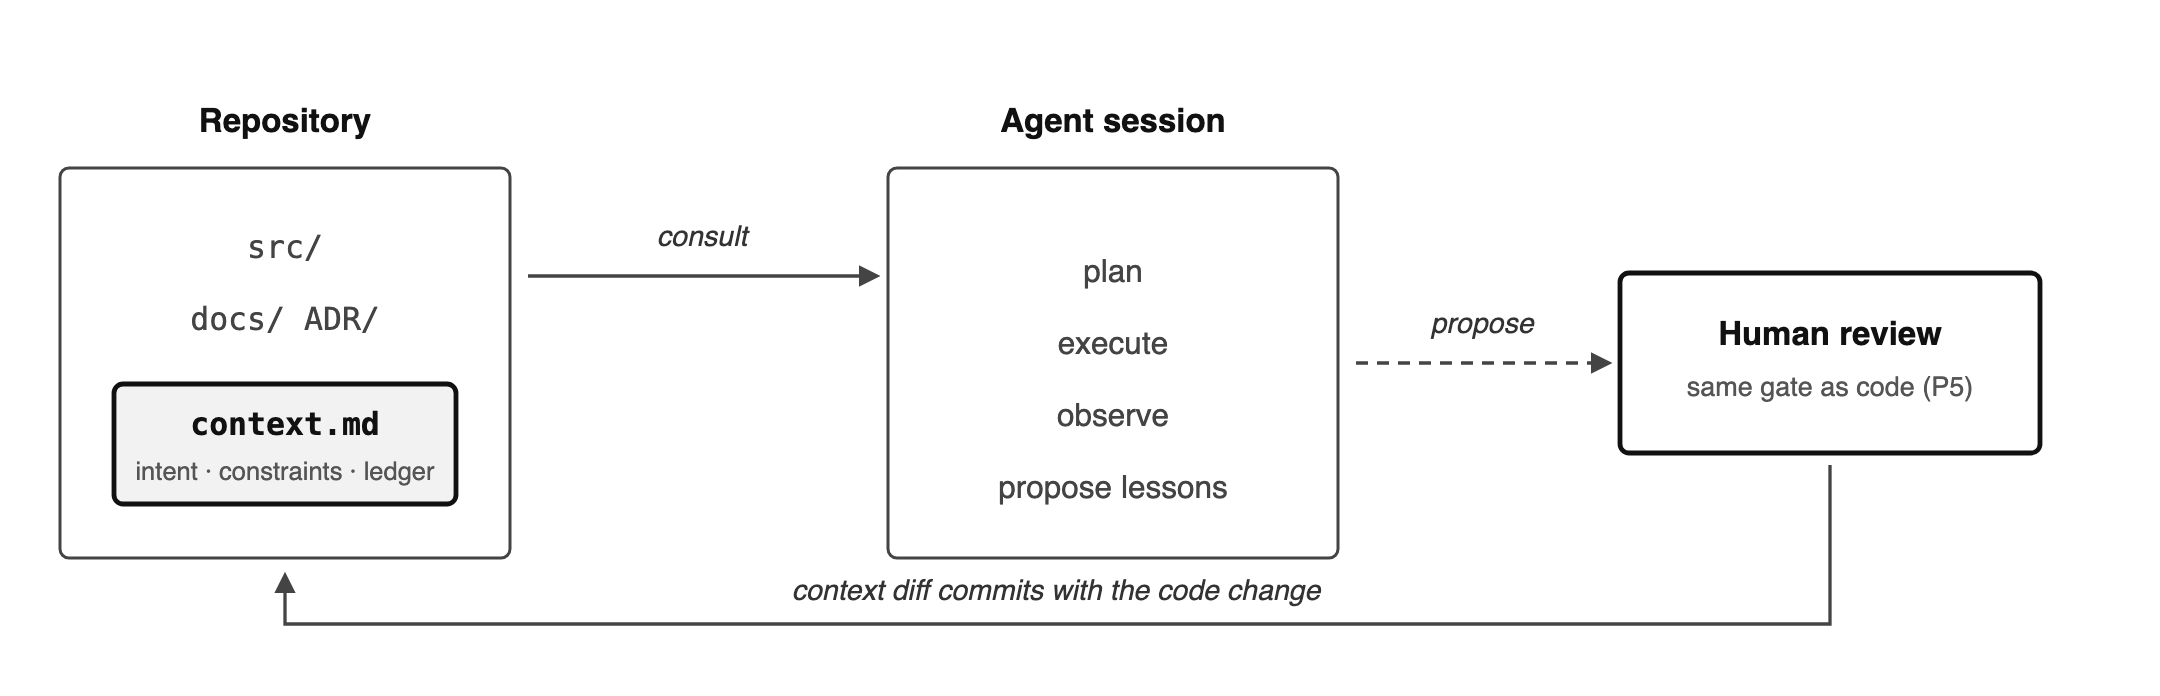
\includegraphics[width=\linewidth]{figures/fig1-architecture.png}
\caption{The Repository Context Layer is added alongside a repository's existing artifacts. An agent consults it before planning and proposes updates after executing; every update travels through the same review as the code that motivated it.}
\label{fig:arch}
\end{figure}

\subsection{Required properties}
An implementation conforms to the architecture if it satisfies six properties. \textbf{P1 Co-versioned:} the context is stored in the repository and follows its branching model. \textbf{P2 Human-readable:} the representation is plain text a maintainer can read and edit without tooling. \textbf{P3 Deterministically discoverable:} an agent locates the context by a fixed rule, not by search (Section~\ref{sec:discovery}). \textbf{P4 Bidirectional:} agents both consume the context and propose additions to it. \textbf{P5 Review-gated:} no change to the context takes effect without passing the project's normal review process. \textbf{P6 Tool-independent:} participation requires only the ability to read and write files.

\subsection{Goals and non-goals}
The layer aims to hold the \emph{operating} knowledge of a project: intent, binding constraints with their reasons, and validated lessons from execution. It is deliberately not a knowledge base of the code itself (the code is present and searchable), not a replacement for retrieval over large corpora, not a record of conversations, and not a configuration system. A useful test: an entry belongs in the layer if a competent new engineer would need to be told it, and would not discover it by reading the code.

\subsection{Relationship to Git}
The architecture makes one load-bearing choice: it defines conventions over plain files in Git rather than a new store. This buys provenance (\texttt{git blame} answers who believed what, and when), review (the pull request is the approval mechanism), branching and rollback (Section~\ref{sec:lifecycle}), distributed synchronization, and audit, all without new infrastructure. The cost is Git's limitations, notably textual rather than semantic merging; Section~\ref{sec:design} discusses the consequences.

\subsection{Four layers}
We separate the pattern into independently adoptable layers: \textbf{L1}, the architecture of this section; \textbf{L2}, the discovery specification of Section~\ref{sec:discovery}; \textbf{L3}, the \ctx{} file format of Section~\ref{sec:format}; and \textbf{L4}, implementations that automate consultation, capture, and retrieval. A team may adopt L1--L3 with no tooling at all; a vendor may implement L1--L2 with a different representation than L3. Conformance claims should name the layers they cover.

\section{The Context Lifecycle}\label{sec:lifecycle}
The lifecycle is the behavioral half of the architecture: it defines when the context is read and when it is written: \emph{consult} $\rightarrow$ \emph{plan} $\rightarrow$ \emph{execute} $\rightarrow$ \emph{observe} $\rightarrow$ \emph{update} $\rightarrow$ \emph{review} $\rightarrow$ \emph{commit}.

\emph{Consult.} Before planning, the agent reads the context in full. Constraints bind the plan; intent breaks ties among admissible designs. \emph{Plan / Execute.} Ordinary agent operation. \emph{Observe.} On completion, the agent asks what the work taught that a future session would otherwise re-learn. Most observations are discarded; durability is the filter. \emph{Update.} Surviving observations are appended to the context's ledger. \emph{Review.} The context diff rides in the same change set as the code, and a human approves both together. \emph{Commit.} The repository's knowledge and behavior advance atomically.

Four invariants summarize the contract. \textbf{I1:} consultation precedes planning. \textbf{I2:} ledger writes are appends. \textbf{I3:} no context change takes effect without review. \textbf{I4:} context changes travel with the code changes that motivated them.

\emph{Branch behavior.} Because the context is a file, it branches when the code branches. A learning made on an experimental branch is visible only there, which is correct: it may be true only there. Deleting an abandoned branch deletes beliefs that were never validated.

\emph{Merge behavior.} Merging a branch merges its context. Appends to a ledger from different branches usually touch different lines and merge cleanly; a union merge strategy makes this explicit. Conflicting edits to a constraint are semantic conflicts, and the architecture deliberately routes them to a human: two branches that learned incompatible things have surfaced a real disagreement.

\emph{Rollback.} Reverting a commit reverts the beliefs recorded in it. This is a feature: if the change that motivated a learning is withdrawn, the learning's justification is withdrawn with it.

\section{Context Discovery Specification}\label{sec:discovery}
Discovery must be deterministic (P3): a fixed path is an API, and an agent must not depend on search or inference to find its own operating contract. The key words MUST, SHOULD, and MAY follow RFC~2119~\cite{rfc2119}. An agent MUST check \texttt{.repo/context.md}, then \ctx{} at the repository root, and use the first file found. The paths \texttt{.repo/context/} and \texttt{context/} (repository root) are RESERVED for sharding of large contexts. Agents encountering either before they support sharding MUST still honor the first rule; a repository that shards SHOULD keep a root context file as the discoverable index into the shards. Agents MUST ignore sections they do not understand and MUST NOT fail on additional files or metadata.

\section{The Context File Format}\label{sec:format}
The default representation (L3) is a single CommonMark file with a top-level \texttt{\#~Repository Context} heading and three required sections, in any order. \emph{Intent} states what the project is and the design philosophy subordinate decisions must serve; it is the tiebreaker among admissible designs. \emph{Constraints} are the binding rules; each entry SHOULD carry its reason, including what was rejected and why. Constraints are edited, not appended. \emph{Evolved Context} is an append-only ledger of dated entries recording what agents and humans learned during execution. Entries are never rewritten; corrections are recorded as superseding entries. Entries that prove durable are \emph{promoted}: moved into Constraints in a reviewed change.

Existing projects rarely start empty. A practical seeding procedure: distill each ADR's decision and consequences into one Constraints entry; move durable guidance out of instruction files; and start the ledger empty. Seeding is a single reviewed commit.

\section{Design Discussion}\label{sec:design}
Five design choices attract consistent pushback; we record the reasoning.

\emph{One file or many?} One file is the default because the context is a working set, not an archive: its purpose is to be read, in full, at the start of every session. When a context genuinely outgrows one file, the reserved directories admit sharding by topic, with the root file retained as the discoverable index. The failure mode to resist is archival creep: a context file that tries to be documentation stops being read.

\emph{Is append-only always right?} Append-only applies to the ledger, not the layer. The ledger is an evidence log; rewriting evidence destroys the provenance that makes it trustworthy. Constraints, by contrast, are current law and are edited in place, with Git history preserving every prior state.

\emph{Merge conflicts.} Textual conflicts concentrate in the ledger, where concurrent appends collide at the file's tail. Declaring a union merge for the context file resolves concurrent appends automatically while leaving edits to shared lines for humans. The architecture automates the merges that cannot be wrong and refuses to automate the ones that can.

\emph{Hierarchical context.} Monorepos want scoped context. The v0.x position is to standardize the root and defer hierarchy, reserving nearest-ancestor discovery as the intended extension. Hierarchy multiplies the spec surface, and the pattern should earn complexity with adoption evidence first.

\emph{Agent write authority and the threat model.} An agent may propose anything and enact nothing. Every context change lands through the same review gate as code (I3), so the ceiling on agent authority equals the rigor of the project's review process. The gate is also the security boundary: a context layer is standing instruction to future agents, making a poisoned entry persistent prompt injection. Three properties contain this: review-gating (P5) means hostile entries must pass a human; provenance (P1) means every entry has an author, a commit, and a motivating change; human-readability (P2) denies attackers obscurity. Reviewers SHOULD treat context diffs with the scrutiny of code diffs, and conformant tooling MUST refuse to promote files that do not explicitly declare themselves context documents. The gate must also scale: an agent attempting dozens of tasks a day would exhaust reviewer attention if every raw lesson demanded fresh scrutiny. Automated pre-screening therefore belongs in front of the human---format and size linting, classifiers that flag privilege-expanding or outward-pointing instructions, and mechanical promotion rules such as the rubric our evaluation uses (Section~\ref{sec:eval})---so the reviewer sees few, well-formed, pre-vetted diffs rather than a stream of candidates. In our evaluation such a rubric screened every candidate lesson with no human in the loop, rejecting roughly one in ten before review.

\section{What the Layer Is Not}
It is not RAG: consultation is by contract, not similarity. It is not prompt engineering: instruction files configure behavior top-down and are static between human edits, while the layer evolves through execution. It is not documentation: docs address human onboarding at human timescales; the layer is machine-facing operating state. And it is not chat memory: platform memories attach to a user or a tool, while repository context attaches to the artifact all users and tools share. The distinctions matter because each framing suggests the wrong lifecycle: archives are allowed to go stale, and this must not.

\section{Reference Implementation and Integrations}\label{sec:impl}
A reference implementation, Metatron~\cite{metatron}, implements all four layers (L1--L4) for teams that want the lifecycle automated: project knowledge as individual Markdown files in an open knowledge format, one decision per file with structured front matter, sharded under a root-level \texttt{context/} directory, with a scaffolded root \ctx{} whose Constraints point into the shards---so discovery works for any conformant agent with no tool-specific knowledge. Candidate entries flow through an explicit review step before becoming canonical. The implementation exists to reduce friction, not to be required: a team using plain \ctx{} with disciplined review conforms to the same architecture.

Current agents need a one-time bootstrap telling them the contract exists; the natural place is the instruction file they already read (\texttt{CLAUDE.md}, \texttt{AGENTS.md}, \texttt{.cursorrules}, or a system-prompt sentence). This yields a clean division of labor: the instruction file tells the agent that the context layer exists; the context layer holds what the agent needs to know. Because every integration reads the same artifact, a repository worked on by three different tools accumulates one shared context rather than three private memories.

\section{Empirical Evaluation}\label{sec:eval}
We evaluate the architecture's central behavioral claims---that repository-carried context measurably changes agent behavior, and that lessons learned in one task transfer to different tasks sharing an underlying constraint---in a pre-registered experiment on SWE-bench Verified~\cite{swebench}. The protocol (hypotheses, conditions, metrics, analysis plan, and a power simulation) was frozen and externally timestamped before any confirmatory run; pilot runs used for feasibility are excluded from confirmatory analysis. All materials---the frozen protocol, blind-authoring audit trails, episode transcripts, promotion logs, and evaluation verdicts---are released for replication~\cite{artifact}.

\subsection{Design}
\emph{Transfer pairs.} SWE-bench Verified supplies real historical bugs, each with a hidden grading test suite and the maintainers' fix (the \emph{gold patch}). We identified \emph{constraint groups}---instances within one repository whose fixes depend on the same convention (e.g., xarray's \texttt{keep\_attrs} propagation; Django's \texttt{deconstruct()} fidelity rules)---and froze ordered transfer pairs $(A,B)$ before any run: $B$ is held out, and the treatment's only advantage on $B$ is context derived from working on $A$. Two pairs are documented regression chains, where the benchmark itself records $B$ re-breaking the constraint $A$'s fix established---the failure mode of Section~1, occurring in the wild. Groups were identified by screening all 500 Verified instances (keyword clustering over problem statements and patch-touched subsystems, then manual confirmation), yielding 12 groups of roughly 40 instances concentrated in three repositories; transfer effects are claimed for this constraint-sharing regime---about 8\% of the benchmark---not benchmark-wide, a scope Section~\ref{sec:eval}.3 revisits.

\emph{Conditions.} Executors: a frontier model (Claude Opus 4.8) and a small local model (Gemma~4, 8B, quantized). Context: none, \emph{seeded} (a static \ctx{}), or \emph{emergent} (an initially empty store accumulating the agent's own promoted lessons through the lifecycle of Section~\ref{sec:lifecycle}). A labeled \emph{oracle-taught} arm, whose learning step sees the gold patch of task $A$ only, bounds attainable lesson quality and is never pooled. Seeded files were authored by fresh model sessions given only a years-old repository checkout (history removed), its documentation, and constraint-group names---never a problem statement, patch, or test; authoring transcripts are released as a blindness audit. All conditions share one minimal scaffold; lessons pass a mechanical promotion rubric (repo-generality verified by a fixed-prompt classifier; instance identifiers, line numbers, and over-length entries rejected deterministically). Gold patches and hidden tests never enter executor or learning prompts. Paired analyses use sign-flip permutation tests per (pair~$\times$~repetition); five repetitions per cell locally, three at the frontier.

\subsection{Results}
\emph{The lifecycle works at frontier capability.} On the initial, mostly-easy pair set the frontier cells were ceiling-invalidated (94.4\% localization unaided), as the pre-registered stratification rule anticipated. On the stratified set---16 pairs across 11 constraint groups, all held-out tasks of ``15 minutes--1 hour'' difficulty or harder---the frontier executor running the full consult--execute--learn--promote loop resolves \textbf{72.9\%} of held-out tasks versus \textbf{58.3\%} without it ($+14.6$\,pp, paired $p=0.041$; localization 91.7\% vs.\ 81.2\%, $p=0.064$; direction positive in 8 of 11 groups; Figure~\ref{fig:slope}). The lessons driving the effect were extracted from the agent's own transcripts under the leakage guards: one task's failure experience, converted into a measurable resolve improvement on different tasks sharing the constraint, at the cost of one learning turn per task.

\begin{figure}[t]
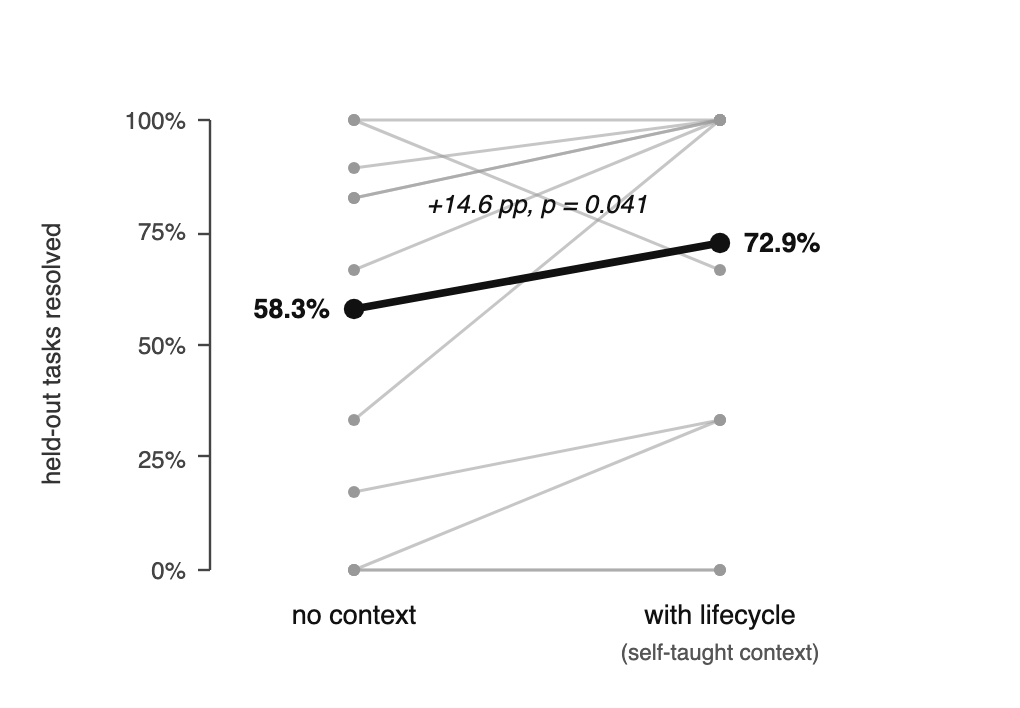
\includegraphics[width=.92\linewidth]{figures/fig2-slopegraph.png}
\caption{Frontier executor resolve rate on held-out tasks, without and with the lifecycle. Gray lines: the 11 constraint groups (one declines); black: overall means.}
\label{fig:slope}
\end{figure}

\emph{Learning from failure beats learning from answers.} A labeled oracle variant---identical to the lifecycle arm except that its lesson-extraction step was additionally shown the maintainers' actual fix for task $A$---produced lessons that did not transfer: 60.4\% resolve, indistinguishable from no context at all ($+2.1$\,pp, $p=1.0$) and directionally worse than the self-taught arm ($-12.5$\,pp, $p=0.067$). The tier inversion is instructive: the small executor benefited most from gold-derived lessons (Figure~\ref{fig:gradient}), the frontier executor only from its own failures. Answer-derived lessons encode solutions; failure-derived lessons encode traps and process---and a capable model needs the latter. What transfers upward in capability is process knowledge, not solution summaries.

\emph{Context pays for itself at the frontier.} The lifecycle arm also spent less: 40.6K versus 49.8K tokens per episode ($-20\%$), and---combining spend with success---\textbf{81.8K $\rightarrow$ 55.7K tokens per resolved task ($-32\%$; Figure~\ref{fig:tokens})}. The decomposition is telling: episodes that ended in a fix cost the same in both arms ($\approx$33.6K); the entire saving comes from avoiding doomed exploration. The small executor shows the opposite sign ($+20\%$ tokens per episode with the seed, $p=0.012$, despite significantly fewer turns): for a strong model, repository context is self-financing; for a weak one it is a paid capability upgrade.

\begin{figure}[t]
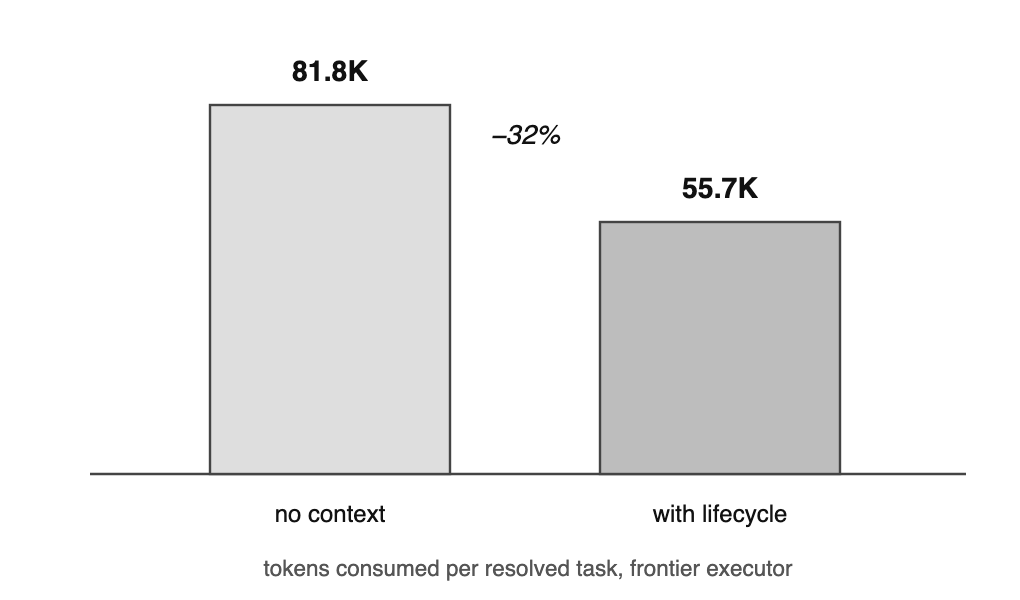
\includegraphics[width=.85\linewidth]{figures/fig4-tokens.png}
\caption{Total tokens spent per successfully resolved task (frontier executor, 48 episodes/arm). Successful episodes cost the same in both arms; the saving comes from fewer failed explorations. The oracle-taught variant spends like the lifecycle arm (64.1K/resolved) without matching its resolve rate.}
\label{fig:tokens}
\end{figure}

\emph{Benefit requires an author more capable than the reader.} With the small local executor held fixed (36 pairs $\times$ 5 repetitions per cell, pooled over the pre-planned pair expansion), held-out-task outcomes vary only with who authored its context (Figure~\ref{fig:gradient}): a blind frontier-authored seed raises gold-file localization from 21.1\% to 47.2\% ($+26.1$\,pp, paired $p<0.0001$) and context distilled from authoritative fixes raises it to 42.8\% ($+21.7$\,pp, $p<0.0001$)---the two are statistically indistinguishable from each other---while the executor's own promoted lessons move nothing ($+0.0$\,pp, $p=1.0$). The effect is a capability threshold, not a dose curve: any author tier above the executor roughly doubles its localization, while self-authorship equals no context exactly. The small model's own promoted lessons---162 across 60 pair-repetitions---transfer nothing: inspection shows it records tooling tactics rather than repository constraints, while the frontier model, under the identical learning prompt, records precisely the constraint-and-localization facts the clusters center on. Localization and episode completion are where the layer moves this executor; its resolve rate does not improve significantly at pooled power. The practical reading: seed and maintain context layers with capable writers (humans, frontier models, distillation from authoritative fixes); weaker local agents then inherit the navigational benefit at zero marginal inference cost---a pattern we call \emph{context inheritance}: one frontier authoring pass, paid once, propagates senior-level navigational knowledge to every cheaper agent working in the repository.

\begin{figure}[t]
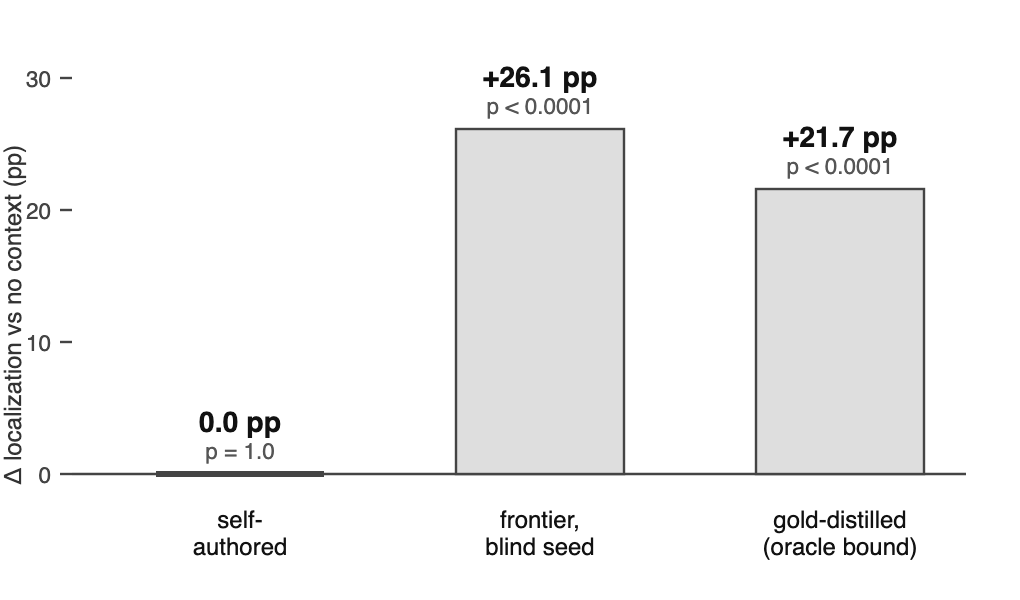
\includegraphics[width=.92\linewidth]{figures/fig3-gradient.png}
\caption{Paired improvement in the 8B executor's gold-file localization over its no-context control, by context author (36 pairs $\times$ 5 repetitions). Resolve-rate deltas are not significant at this tier (oracle $+2.2$\,pp, $p=0.22$).}
\label{fig:gradient}
\end{figure}

The whole experiment---roughly 1,800 episodes and 750 containerized evaluations across seven conditions---consumed under \$200 of frontier-API spend, consistent with the layer's economic premise: expensive knowledge, written once, read cheaply forever.

\subsection{Threats to Validity}
Localization is a proxy for working in the right place, not for correctness; resolve rates are reported alongside. Training contamination affects both arms of every within-model comparison symmetrically and compresses deltas toward zero. The orchestrating researcher session had instance exposure and was excluded from seed authorship and lesson selection (blind sessions and a mechanical rubric, respectively). Three repositories, one benchmark, one scaffold; transfer pairs target constraint-shaped bugs by construction. This scope is construct validity rather than sampling bias: recurring constraints are definitionally the only setting in which shared context can pay off, so the constraint-sharing regime (about 8\% of Verified) is the setting the architecture is designed for---and the two documented regression chains in our sample show the regime arises naturally in real projects, not only under our selection. A resolve-rate improvement for the local executor that was marginal in the initial pair set ($p=0.066$) did not survive the pre-planned pair expansion (pooled $p=0.22$) and is not claimed. Oracle-taught arms are labeled bounds outside the confirmatory families, and the frontier failure-versus-answers contrast is marginal ($p=0.067$)---reported as directional.

\section{Future Work}
\emph{Validation:} conformance linting for the format and, more usefully, the lifecycle: CI integrations (e.g., a pull-request action producing semantic context-diff summaries) that flag substantive changes landing with no context diff over long periods. \emph{Semantic merging:} LLM-assisted reconciliation of contradictory ledger entries, proposed to the human rather than applied. \emph{Summarization and budgets:} automatic distillation of aging ledgers. \emph{Hierarchy:} the nearest-ancestor extension. \emph{Cross-repository inheritance:} organization-wide constraint layers member repositories extend. \emph{Extended efficacy measurement:} Section~\ref{sec:eval} establishes transfer within constraint-sharing pairs; open questions include accumulation dynamics over long task sequences and effects in longitudinal deployments.

\section{Conclusion}
Software repositories already version their code, their tests, their documentation, and their infrastructure. This paper has argued---and now measured---that they should also version their operating context: a small, human-readable, review-gated store that agents consult before planning and improve after executing. The architecture asks for no new infrastructure, reuses the trust machinery of Git and code review, and degrades gracefully to a single Markdown file maintained by hand. Its contested choices all follow from one principle: the layer must remain small enough to read, legible enough to review, and trustworthy enough to obey. The pre-registered evaluation gives the pattern its first controlled evidence: the lifecycle converts an agent's failure experience into transferable operating knowledge, cuts the token cost of a fixed bug by a third, and the layer's value scales with the capability of its authors. Software engineering standardized version control for code; AI-native software engineering will require versioning shared operating knowledge as well.

\section*{Data Availability}
Every empirical claim in this paper is reproducible from released materials~\cite{artifact}: the pre-registration frozen at a verifiable git tag \emph{before} any confirmatory run; the seed-authoring transcripts proving blindness; the complete harness (agent scaffold, learning prompts, mechanical promotion rubric, batch orchestration); every episode's predictions, promotion decisions, and containerized evaluation verdict; and the analysis scripts. A one-command entry point (\texttt{make docker-reproduce}) recomputes all fifteen numbers reported here from the raw run data and verifies each against the text, with no network access and no model inference required; second and third tiers of the runbook re-run individual episodes and full arms. Evaluation uses the benchmark's official container images.

\begingroup\small\vspace{-2pt}
\begin{thebibliography}{9}
\bibitem{manifesto} P.~Kerbel. ``The Repository Context Layer: The Missing Layer of Agentic Software Development,'' manifesto and specification repository, 2026. \url{https://github.com/kerbelp/repository-context-layer}.
\bibitem{lewis2020rag} Patrick Lewis, Ethan Perez, Aleksandra Piktus, et al. 2020. Retrieval-Augmented Generation for Knowledge-Intensive NLP Tasks. In \emph{Advances in Neural Information Processing Systems 33 (NeurIPS 2020)}. Curran Associates.
\bibitem{mcp2024} Anthropic. 2024. Introducing the Model Context Protocol. Retrieved July 2026 from \url{https://modelcontextprotocol.io}.
\bibitem{nygard2011adr} Michael Nygard. 2011. Documenting Architecture Decisions. Retrieved July 2026 from \url{https://cognitect.com/blog/2011/11/15/documenting-architecture-decisions}.
\bibitem{rfc2119} Scott Bradner. 1997. Key Words for Use in RFCs to Indicate Requirement Levels. IETF RFC 2119. \url{https://doi.org/10.17487/RFC2119}.
\bibitem{shinn2023reflexion} Noah Shinn, Federico Cassano, Ashwin Gopinath, Karthik Narasimhan, and Shunyu Yao. 2023. Reflexion: Language Agents with Verbal Reinforcement Learning. In \emph{Advances in Neural Information Processing Systems 36 (NeurIPS 2023)}.
\bibitem{wang2023voyager} Guanzhi Wang, Yuqi Xie, Yunfan Jiang, et al. 2024. Voyager: An Open-Ended Embodied Agent with Large Language Models. \emph{Transactions on Machine Learning Research} (2024). arXiv:2305.16291.
\bibitem{packer2023memgpt} Charles Packer, Sarah Wooders, Kevin Lin, et al. 2023. MemGPT: Towards LLMs as Operating Systems. arXiv:2310.08560.
\bibitem{park2023generative} Joon Sung Park, Joseph O'Brien, Carrie Jun Cai, Meredith Ringel Morris, Percy Liang, and Michael S. Bernstein. 2023. Generative Agents: Interactive Simulacra of Human Behavior. In \emph{Proceedings of the 36th Annual ACM Symposium on User Interface Software and Technology (UIST '23)}. ACM. \url{https://doi.org/10.1145/3586183.3606763}.
\bibitem{swebench} C.~E. Jimenez et al. 2024. SWE-bench: Can Language Models Resolve Real-World GitHub Issues? In \emph{The Twelfth International Conference on Learning Representations (ICLR 2024)}. \url{https://openreview.net/forum?id=VTF8yNQM66}. SWE-bench Verified: human-validated subset, 2024.
\bibitem{metatron} P.~Kerbel. ``Metatron: a files-first repository context layer for AI coding agents,'' software, v0.12.0, 2026. \url{https://github.com/kerbelp/metatron}.

\bibitem{artifact} P.~Kerbel, M.~Kerbel, V.~Abramov, and L.~Abramov. ``RCL efficacy study: replication artifacts,'' 2026. \artifact.
\end{thebibliography}
\endgroup

\end{document}
